\documentclass[11pt, oneside]{article} 
\usepackage{geometry}
\geometry{letterpaper} 
\usepackage{graphicx}
	
\usepackage{amssymb}
\usepackage{amsmath}
\usepackage{parskip}
\usepackage{color}
\usepackage{hyperref}

\graphicspath{{/Users/telliott_admin/Tex/png/}}
% \begin{center} 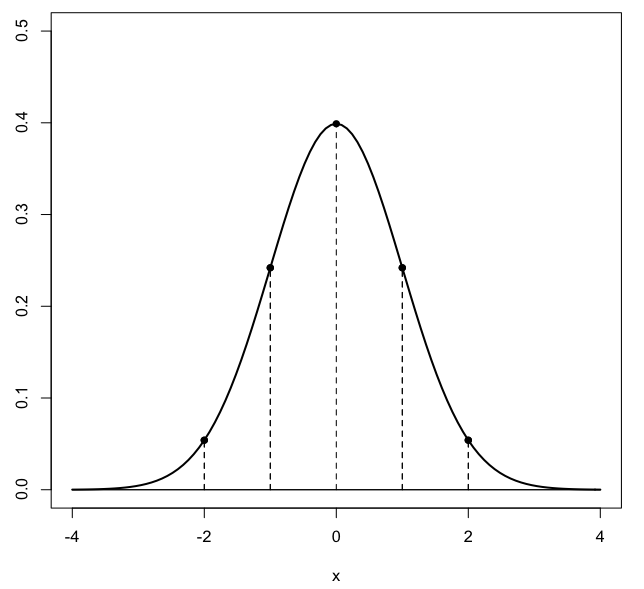
\includegraphics [scale=0.4] {gauss3.png} \end{center}

\title{Intermediate Value Theorem}
\date{}

\begin{document}
\maketitle
\Large

\section{Intermediate Value Theorem}

Above we had Bolzano's Theorem:

If $f$ is continuous on $[a,b]$ and $f(a) < 0 < f(b)$ then there is some $x$ in $[a,b]$ such that $f(x) = 0$.

We want to show that $f(x)$ achieves some arbitrary value $c$ between its maximum and minimum values.

\subsection*{Proof}

Define $g(x) = f(x) - c$.  It is easy to show that if $f$ is continuous so is $g$.  Then, there is some $x$ in $[a,b]$ such that $g(x) = 0 = f(x) - c$.  Thus, there is some $x$ in $[a,b]$ such that $f(x) = c$.

\end{document}}